% Command Succession with a Hostile Commander.
%
% The text of this draft follows the writing rules of ASD-STE100 (Simplified Technical
% English). See STE.md, and run `python3 scripts/ste_check.py` after each change.
%
% Format switch. \srdstrue gives the IEEE conference format (the format of SRDS).
% \srdsfalse gives the ACM acmsmall format (the format of ACM TCPS). The section files are
% the same for the two formats.
\newif\ifsrds
\srdstrue
% SRDS has double-blind review. Set \anontrue before a submission to hide the authors.
\newif\ifanon
\anonfalse

\ifsrds
  \documentclass[conference]{IEEEtran}
  \usepackage[T1]{fontenc}
  \usepackage{amsmath,amssymb}
  % IEEEtran has a proof environment of its own. Remove it, then load amsthm.
  \let\proof\relax
  \let\endproof\relax
  \usepackage{amsthm}
  \usepackage{xcolor}
  \usepackage{cite}
  \usepackage[hidelinks]{hyperref}
\else
  % `review` adds line numbers for comments; remove it for a submission.
  \documentclass[acmsmall,review]{acmart}
  \setcopyright{none}
  \settopmatter{printacmref=false}
  \renewcommand\footnotetextcopyrightpermission[1]{}
  \acmJournal{TCPS}
\fi

\usepackage{booktabs}
\usepackage{tabularx}
\usepackage{tikz}
\usetikzlibrary{arrows.meta,calc,decorations.pathreplacing,patterns}
\usepackage[nameinlink,noabbrev,capitalise]{cleveref}

\hypersetup{
  pdftitle={Command Succession with a Hostile Commander},
  pdfauthor={Aditya Sissodiya, Eric Chiquito, Johan Kristiansson, Ulf Bodin},
  pdfsubject={Working draft (not for submission)},
}
\pdfinfoomitdate=1
\pdftrailerid{}

% Theorem environments with names of their own, so that the two formats give the same result.
\theoremstyle{plain}
\newtheorem{thm}{Theorem}
\newtheorem{lem}{Lemma}
\newtheorem{cor}{Corollary}
\newtheorem{prp}{Proposition}
\theoremstyle{definition}
\newtheorem{dfn}{Definition}
\crefname{thm}{Theorem}{Theorems}
\crefname{lem}{Lemma}{Lemmas}
\crefname{cor}{Corollary}{Corollaries}
\crefname{prp}{Proposition}{Propositions}
\crefname{dfn}{Definition}{Definitions}

% Colors for the figures and for the draft notes.
\definecolor{accept}{HTML}{5B8DB8}
\definecolor{fence}{HTML}{C47B2C}
\definecolor{ink}{HTML}{1F2A44}
\definecolor{soft}{HTML}{EEF2F8}
\definecolor{warn}{HTML}{C0392B}

% Draft notes: \pending shows work that is not done. Remove each note before a submission.
\newcommand{\pending}[1]{\textcolor{fence}{[\textit{#1}]}}

% The name of the protocol. The name is not final.
\newcommand{\sys}{\textsc{Mandate}}
% Certificates: a grant and a renewal.
\newcommand{\grant}[1]{\mathsf{G}\langle #1\rangle}
\newcommand{\renew}[1]{\mathsf{R}\langle #1\rangle}
\newcommand{\eps}{\varepsilon}
% The name of a file in the repository.
\newcommand{\file}[1]{\nolinkurl{#1}}  % a file name; lines can break at the slashes

% Numbers from the testbed of the previous draft (a model without a hostile officer).
% Generated by `python -m aas_testbed latex` (rescue-ois testbed, exporter commit 01e1a681c882),
% from results generated by commit 705c1874cae3. Do not edit; re-run the exporter.

\newcommand{\tbSearchRevoked}{0}
\newcommand{\tbSearchMisclassified}{0}
\newcommand{\tbSeedsPerCell}{20}
\newcommand{\tbSearchRuns}{2{,}200}
\newcommand{\tbRelayOverlap}{107\,s}
\newcommand{\tbRelayResidual}{1}
\newcommand{\tbRelayOverlapAcked}{0\,s}
\newcommand{\tbFlapOverlapRuns}{8}
\newcommand{\tbFlapRuns}{60}
\newcommand{\tbFlapOverlapRunsAcked}{0}
\newcommand{\tbFlapRunsAcked}{30}
\newcommand{\tbStrictLostNeverMin}{24}
\newcommand{\tbStrictLostNeverMax}{31}
\newcommand{\tbClosingSettlePninetyfive}{7\,s}
\newcommand{\tbSFourSettlePninetyfiveKept}{747\,s}
\newcommand{\tbSFourNeverSettledLost}{24}
\newcommand{\tbSignedResidual}{17}
\newcommand{\tbSignedFlips}{51}
\newcommand{\tbAcceptedResidual}{0}
\newcommand{\tbAcceptedFlips}{0}
\newcommand{\tbAcceptedOverlap}{2\,s}
\newcommand{\tbPBNoCommand}{1{,}111\,s}
\newcommand{\tbPBRefused}{19}
\newcommand{\tbSThreeLNoCommand}{1{,}112\,s}
\newcommand{\tbSThreeLOverlapLong}{119\,s}
\newcommand{\tbSOneOverlapFast}{73\,s}
\newcommand{\tbSFourAWindow}{238\,s}
\newcommand{\tbSFourTakeover}{299\,s}
\newcommand{\tbSFourGap}{61\,s}
\newcommand{\tbSFiveOverlap}{902\,s}
\newcommand{\tbSFiveResidual}{15}
\newcommand{\tbSThreeSilentOverlap}{1{,}022\,s}
\newcommand{\tbSThreeSilentResidual}{16}
\newcommand{\tbUnfitSOne}{302\,s}
\newcommand{\tbUnfitSThree}{362\,s}
\newcommand{\tbUnfitSFourPerson}{300\,s}
\newcommand{\tbUnfitSFourNoCommand}{1{,}200\,s}
\newcommand{\tbMuteOverlap}{1\,s}
\newcommand{\tbDeafNoCommand}{962\,s}
\newcommand{\tbHandoverResidual}{16}
\newcommand{\tbHandoverOverlap}{903\,s}
\newcommand{\tbDoubtTen}{2}
\newcommand{\tbDoubtSixty}{9}
\newcommand{\tbBlindSixty}{0}
\newcommand{\tbBlindThreeHundred}{5}
\newcommand{\tbBlindTwelveHundred}{21}
\newcommand{\tbTotalRuns}{8{,}950}
\newcommand{\tbMarginPlainLast}{8\,s}
\newcommand{\tbMarginAckedFirst}{1\,s}


\begin{document}

\ifsrds
  \title{Command Succession with a Hostile Commander:\\
  Tenure Limits when an Attacker Controls the Links}
  \ifanon
    \author{\IEEEauthorblockN{Authors hidden for review}}
  \else
    \author{\IEEEauthorblockN{Aditya Sissodiya, Eric Chiquito, Johan Kristiansson and Ulf Bodin}
    \IEEEauthorblockA{Department of Computer Science, Electrical and Space Engineering\\
    Lule{\aa} University of Technology, Lule{\aa}, Sweden\\
    \{aditya.sissodiya, eric.chiquito, johan.kristiansson, ulf.bodin\}@ltu.se}}
  \fi
  \maketitle
  \begin{abstract}
  An operator who controls field devices through a network must continue to give orders when
links have failures. But a device that obeys an isolated operator cannot know if the operator is
loyal. It is possible that an attacker has the key of the operator and cut the links. In the
2015 attack on the Ukrainian power grid, attackers opened breakers from the consoles of the
operators. We examine how command stops, and how command goes to a different person, when
the commander can be hostile and the attacker controls all links.

First, we show a limit. For each protocol, a hostile commander keeps a device for a time
not less than the outage that a loyal commander can continue through. The same
argument applies to a deputy who gets command on a timeout.

Second, we give a protocol, \sys{}. Command expires at a time that each device compares
with its clock, unless a quorum of officers signs a renewal. A specified number of loyal
officers always removes a commander, and hostile officers cannot remove a commander without
loyal officers. \sys{} is near the limit. The difference is not more than the sum of the
renewal interval, the collection time and six clock errors.

Third, we give the cost of \sys{} as formulas and compare it with four known designs. The
paper has the proofs. A model check of the rules and a simulation with a hostile commander
are not done at this time.

  \end{abstract}
  \begin{IEEEkeywords}
  command authority, succession, Byzantine faults, leases, revocation, intrusion tolerance,
  SCADA, power grid
  \end{IEEEkeywords}
\else
  \title[Command Succession with a Hostile Commander]{Command Succession with a Hostile
  Commander: Tenure Limits when an Attacker Controls the Links}
  \author{Aditya Sissodiya}
  \email{aditya.sissodiya@ltu.se}
  \author{Eric Chiquito}
  \email{eric.chiquito@ltu.se}
  \author{Johan Kristiansson}
  \email{johan.kristiansson@ltu.se}
  \author{Ulf Bodin}
  \email{ulf.bodin@ltu.se}
  \affiliation{%
    \institution{Lule{\aa} University of Technology}
    \department{Department of Computer Science, Electrical and Space Engineering}
    \city{Lule{\aa}}
    \postcode{SE-971 87}
    \country{Sweden}}
  \renewcommand{\shortauthors}{Sissodiya et al.}
  \begin{abstract}
  An operator who controls field devices through a network must continue to give orders when
links have failures. But a device that obeys an isolated operator cannot know if the operator is
loyal. It is possible that an attacker has the key of the operator and cut the links. In the
2015 attack on the Ukrainian power grid, attackers opened breakers from the consoles of the
operators. We examine how command stops, and how command goes to a different person, when
the commander can be hostile and the attacker controls all links.

First, we show a limit. For each protocol, a hostile commander keeps a device for a time
not less than the outage that a loyal commander can continue through. The same
argument applies to a deputy who gets command on a timeout.

Second, we give a protocol, \sys{}. Command expires at a time that each device compares
with its clock, unless a quorum of officers signs a renewal. A specified number of loyal
officers always removes a commander, and hostile officers cannot remove a commander without
loyal officers. \sys{} is near the limit. The difference is not more than the sum of the
renewal interval, the collection time and six clock errors.

Third, we give the cost of \sys{} as formulas and compare it with four known designs. The
paper has the proofs. A model check of the rules and a simulation with a hostile commander
are not done at this time.

  \end{abstract}
  % Concepts selected by hand; make them again with the ACM CCS tool before a submission.
  \ccsdesc[500]{Computer systems organization~Dependable and fault-tolerant systems and networks}
  \ccsdesc[500]{Security and privacy~Access control}
  \ccsdesc[300]{Computer systems organization~Embedded and cyber-physical systems}
  \keywords{command authority, succession, Byzantine faults, leases, revocation, intrusion
  tolerance, SCADA, power grid}
  \maketitle
\fi

\noindent\pending{Draft of 11 November 2026. Text in this color shows work that is not
done. The supervisors did not give their approval for the problem, the grid example, or the
venue at this time.}

\section{Introduction}
\label{sec:intro}

Many systems give one person the authority to control devices at a distance. An operator in
the control center of a power company opens and closes breakers in substations. In this
paper, \emph{command} is this authority, and the \emph{commander} is the person who has it.
The devices get the orders through a network, and networks have failures. Thus the devices
must continue to obey a commander who is isolated from the other parties.

This property has a cost. A device that obeys an isolated commander cannot know the cause
of the outage. A link failure and an attack give the device the same messages. In the
attack, an attacker gets the key of the commander and then cuts the links to the other
parties. The device continues to obey, and the other parties cannot tell it to stop.

The attack on three Ukrainian power companies in December 2015 had these two
parts~\cite{eisac2016ukraine}. The attackers used the consoles of the operators to open
breakers in 27 or more substations, and approximately 225{,}000 customers had no
power~\cite[p.~8]{eisac2016ukraine}. The attackers also cut the remote control. The report
records that ``even if the operator workstations were recovered, remote commands could not
be issued to bring the substations back online''~\cite[p.~9]{eisac2016ukraine}. We use this
attack only as an example. The report does not tell if the orders had signatures.

A second attack uses the succession rule. Many systems give command to a deputy when no
message comes from the commander for a specified time. An attacker who controls the links
can stop the messages of a loyal commander until this timeout occurs. Then the deputy gets
command. If the attacker knows the key of the deputy, the attacker has command. In this
paper, the name of this attack is the \emph{timeout attack}.

\paragraph{Problem}
How does command stop, and how does it go to a different person, when the commander can be
hostile and the attacker controls all links? A solution must have three properties. First,
a loyal commander continues through an outage. Second, a hostile commander does not keep
command after the other officers stop their consent. Third, a timeout does not give command
to a hostile deputy.

The first result of this paper shows that a protocol cannot fully have
the first two properties together. It also gives the relation between them.

\paragraph{Known methods}
Byzantine agreement started with a commander who ``need not be
loyal''~\cite[p.~384]{lamport1982byzantine}. But its protocols give a leader no authority
without a quorum~\cite{castro1999pbft}, and a commander must make decisions without a quorum
during an outage. Control systems for the power grid tolerate hostile servers, but not a
hostile operator~\cite{babay2018spire}. Command authentication examines one order at a
time~\cite{mashima2019delaying}. Leases and credentials with a short life give a maximum for
the time that authority stays after revocation~\cite{gray1989leases,zhou2026hrcred}. We
found no work that gives a minimum, and no succession rule that is safe against the timeout
attack (\cref{sec:related}).

\paragraph{Method}
The work has four steps. First, we did a search of the literature with 15 queries and
examined 300 records (\cref{sec:related}). Second, we made a model in which the attacker
controls all links and knows the keys of some officers (\cref{sec:model}). Third, we
compared runs that give a device the same messages, to find limits that apply to all
protocols (\cref{sec:limits}). Fourth, we made a protocol for this model, wrote proofs of
its properties, and calculated its cost (\cref{sec:protocol,sec:analysis,sec:cost}).

\paragraph{Results}
The paper has four results.
\begin{enumerate}
  \item \emph{A limit for the commander} (\cref{thm:limit}). For each protocol, the tenure
  of a hostile commander at a device is not less than the outage tolerance at that device.
  The result applies to limits on time and to limits on the number of orders.
  \item \emph{A limit for the deputy} (\cref{thm:deputy}). The period that a deputy gets on
  a timeout is also the period that an attacker with the key of the deputy gets.
  \item \emph{A protocol} (\cref{sec:protocol}). In \sys{}, a quorum of officers signs each
  renewal of command, and each device compares the end time with its clock. No message to a
  device is necessary to remove a commander. We show unity of command, a maximum for the
  tenure, and a minimum for the outage tolerance
  (\cref{thm:unity,thm:tenure,thm:tolerance}).
  \item \emph{The cost} (\cref{sec:cost}). We give the time without command and the number
  of signatures as formulas, and we compare \sys{} with four known designs.
\end{enumerate}

\paragraph{When to use the results}
The results apply when three conditions are correct. First, one person at a time controls
the devices. Second, the links between that person and the other officers can
have long outages. Third, a hostile commander can cause damage that is not easy to repair.
If outages are short, a quorum for each order is safer. If no officer can be hostile, a
lease from one server is sufficient (\cref{sec:select}).

\paragraph{Work that is done and work that is not done}
\Cref{tab:status} gives the method that shows each result, and the work that is not done.
The proofs are in this paper, but a second person did not examine them at this time. No
result of this paper comes from a test on a power grid.

\begin{table}[t]
\caption{Results and the method that shows each result. The last column tells if the work
is done at this time.}
\label{tab:status}
\centering
\small
\begin{tabularx}{\columnwidth}{@{}>{\raggedright\arraybackslash}X>{\raggedright\arraybackslash}p{0.30\columnwidth}l@{}}
\toprule
Result & Method & Done \\
\midrule
Limits (\cref{thm:limit,thm:deputy}) & Proof & Yes \\
Properties of \sys{} (\cref{thm:unity,thm:tenure,thm:tolerance}, \cref{prp:fallback}) & Proof & Yes \\
Rules of \sys{} & Random tests (\cref{sec:random}) & Yes \\
Rules of \sys{} & Model check & No \\
Cost of \sys{} & Formulas & Yes \\
Cost of expiry and of timeouts with no attacker & Simulation, previous model & Yes \\
Cost with a hostile commander & Simulation & No \\
Local control (rule D3) & Check by a power engineer & No \\
Related work & Abstracts of 300 records & Yes \\
Related work & Full text of each source & No \\
\bottomrule
\end{tabularx}
\end{table}

The paper has these parts. \Cref{sec:background} gives the background, and
\cref{sec:related} the related work and the open problems. \Cref{sec:model} gives the model,
and \cref{sec:limits} the limits. \Cref{sec:protocol,sec:analysis} give the protocol and
its analysis. \Cref{sec:cost} gives the cost and the tests, and \cref{sec:discussion} the
discussion.

\section{Background}
\label{sec:background}

\subsection{Command in a Power Grid}

A power company controls its substations from a control center. An operator at a console
sends orders through the SCADA system to devices in the substations. A typical order opens
or closes a breaker. One operator controls many substations. In the 2015 attack, the
attackers ``operated numerous sites under the control of the
dispatcher''~\cite[p.~14]{eisac2016ukraine}.

The same order can be correct or dangerous. An operator opens a breaker to isolate a fault
or to let personnel do work on equipment. An attacker opens the same breaker to remove
power from customers. The device gets the same order in the two conditions. An analysis
with a model shows the possible effect of such orders on many substations~\cite{ten2018impact}.

Substations also have local control. A person at the substation can operate the equipment
without the network. After the 2015 attack, the companies had ``to move to manual
operations''~\cite[p.~v]{eisac2016ukraine}. \pending{Not done at this time: a power
engineer must examine the text about local control in this paper.}

\subsection{The 2015 Attack and the Model}

Three facts of the attack are in the model of this paper. First, the attackers had the
authority of the operators. They were in the networks of the companies ``for six months or
more''~\cite[p.~3]{eisac2016ukraine}, and they used the consoles of the operators. Second,
the attackers controlled the channels. The report gives steps to ``take control of the
operator workstations and thereby lock the operators out of their
systems''~\cite[p.~8]{eisac2016ukraine}. It also records ``thousands of calls'' to the
call center of a company~\cite[p.~2]{eisac2016ukraine}.

Third, the attackers were not at the substations. The companies moved to manual operations.
An analysis of two subsequent software attacks on power grids is
in~\cite{salazar2024industroyers}.

\Cref{tab:names} gives the names that this paper uses and their equivalents in the grid
example. The model is not only for a grid. It applies to each system in which one person at
a time controls devices through a network.

\begin{table}[t]
\caption{Names in this paper and their equivalents in the grid example. A power engineer
did not examine the right column at this time.}
\label{tab:names}
\centering
\small
\begin{tabularx}{\columnwidth}{@{}l>{\raggedright\arraybackslash}X@{}}
\toprule
Name & Equivalent in the grid example \\
\midrule
Commander & The operator who has authority for an area of the grid \\
Officer & A person who can be the operator for that area, or who gives approval to an operator \\
Deputy & The officer who gets command if the commander stops \\
Device & The equipment in a substation that does the orders \\
Order & A signed message, for example to open a breaker \\
Local control & A person at the substation operates the equipment \\
\bottomrule
\end{tabularx}
\end{table}

\section{Related Work and Open Problems}
\label{sec:related}

\subsection{Method of the Search}
\label{sec:search-method}

We did the search on 10 November 2026 with the Consensus search engine.
We used 15 queries. For each query we examined the first 20 records, thus 300 records in
total. \Cref{app:search} gives the queries. We read the title and the abstract of each
record. We kept a record if its abstract has one or more of the six properties that follow.

\begin{description}
  \item[A] One party makes decisions without a quorum during an outage.
  \item[S] The work has a succession rule.
  \item[H] The party with authority can be hostile.
  \item[L] The attacker controls the links, and thus the timeouts.
  \item[R] Removal tolerates hostile officers, and no message to the device is necessary.
  \item[T] The work gives a limit on the time that authority stays after removal.
\end{description}

We read parts of the full text of four sources only. Two are the paper on the Byzantine
generals problem~\cite{lamport1982byzantine} and the report on the 2015
attack~\cite{eisac2016ukraine}. The other two are the first section
of~\cite{babay2018spire} and pages 1 to 7 of~\cite{bommareddy2024compound}. For these
sources, the paper gives text from the source. The data about all other sources come from
their abstracts. \pending{Not done at this
time: read the full text of each source in \cref{tab:position}.}

\subsection{Five Groups of Work}

\paragraph{Byzantine agreement and replication}
The Byzantine generals problem has a commander who ``need not be
loyal''~\cite[p.~384]{lamport1982byzantine}. Its solutions make the loyal generals agree on
one order. They do not stop a hostile commander who gives the same dangerous order to all
generals. Replication protocols~\cite{castro1999pbft,castro2002pbft,amir2011prime} and
Byzantine quorum systems~\cite{malkhi1998byzquorum} give a leader no authority without a
quorum. A commander is different: the commander must make decisions without a quorum during
an outage.

Other work in this group is near the problem. One protocol puts a limit on the writes of a
hostile client after its removal~\cite{liskov2006byzclients}. Work on a change of the set of
servers makes a previous set safe after the change~\cite{kuznetsov2022reconfig}. Attacks on
timeouts are known. An attacker who delays messages causes incorrect timeouts and a change
of leader~\cite{tennage2023quepaxa,giuliari2024dos}. In replication, the new leader has no
authority without a quorum, thus the damage is to speed and not to safety.

\paragraph{Control systems for the grid that tolerate intrusion}
One group of designs replicates the SCADA server and tolerates hostile
copies~\cite{kirsch2014survivable,babay2018spire,babay2019deploying}. Subsequent work adds
substations~\cite{bommareddy2022realtime} and isolated sites~\cite{bommareddy2024compound}.
The operator stays loyal in this work. The authors of Spire write: ``Note that our threat
model does not cover a compromised HMI or a rogue operator''~\cite{babay2018spire}.

The work of 2024 gives the condition of the removal problem for servers. In automatic
removal, it records that ``compromised entities may try to exploit the reconfiguration
mechanism''~\cite{bommareddy2024compound}. For systems in which a quorum of servers removes
a server, it records that ``the voting criteria is left
undefined''~\cite{bommareddy2024compound}. This text is about servers. We found no
equivalent rule for the person who gives the orders.

\paragraph{Authentication of orders and access of operators}
Signatures show the sender of an
order~\cite{saxena2018signature,amoah2015dnp3,esiner2023provenance}. Other methods compare
the contents of an order with a simulation of the grid before the device obeys
it~\cite{meliopoulos2016command,mashima2018onthefly,mashima2019delaying,hong2019resilient}.
Access control for operators puts a limit on the substations that an operator
controls~\cite{nasr2018operator,nasr2024authorization}. Two designs of 2026 add a second
factor for an order~\cite{ahmad2026gridlogic} or a quorum of operators for a software
change~\cite{pawar2026certiflash}.

These methods examine one order: the sender and the contents. They do not examine if the
sender has command at this time, and they have no succession rule. A check of the contents
cannot reject an order that a loyal commander also gives (\cref{sec:limits}).

\paragraph{Leases, expiry and revocation}
A lease gives authority for a specified time~\cite{gray1989leases}. Three methods make sure that an access decision uses only new
data~\cite{stubblebine1995recent,krishnan2008stale,shakarami2019refresh}. Threshold methods
let a group of nodes give and revoke certificates in a network with no
server~\cite{zhou1999securing,luo2004ursa,liu2013ccrvc}. A survey gives the revocation methods for certificates on the
web~\cite{kwon2025revocation}. A second survey records that a check with no connection is
an open problem~\cite{lee2026ssirevocation}. One design gives a signed proof that a
credential was correct at a point in time~\cite{abraham2020revocable}.

HRCred is the nearest work that we found~\cite{zhou2026hrcred}. A threshold of parties
signs credentials with a short life for each epoch. Its authors show a maximum for the time
that a device accepts a credential after revocation. The credentials are for the identity
of a device. The abstract gives no succession rule and no minimum.

Some results show that two properties cannot be correct together, but they give no
quantity. The CAP result shows that a system
with a partition cannot have consistency and availability
together~\cite{gilbert2002cap,brewer2012cap}. An equivalent result is known for systems
that control equipment~\cite{lee2023cal}. Access control without a quorum makes decisions with
the data that a party has~\cite{jacob2025eventually,yanakieva2021impossibility}. Three
preprints examine the time at which authorization
stops~\cite{santosgrueiro2026effect,parakhin2026bureaucracy,deochake2026heartbeat}.

\paragraph{Handover between persons, and nuclear command}
Work on handover examines how control moves between operators, and between a person and an
automatic
system~\cite{flemisch2012balance,abbink2012haptic,grindley2024handover,nilsen2018handing,marot2022perspectives}.
All parties are loyal in the 20 records of that query. Nuclear command and control has the
two properties of this paper. An order must always go out when the correct authority gives it,
and it must not go out without that
authority~\cite{feaver1992guarding,crawford2025nc3}. A deputy with authority given before
the attack is one known solution~\cite{twigge1999learning}. This work gives the problem,
but it has no protocol model and no attacker on the links.

\begin{table*}[t]
\caption{Related work and the six properties of \cref{sec:search-method}. The entry ``part''
tells that the work has the property for a different party, or has only a part of it. We
made the entries from abstracts, and from text of the sources for the first and the third
row. A person must examine each entry against the full text.}
\label{tab:position}
\centering
\small
\begin{tabular}{@{}lcccccc@{}}
\toprule
Work & A & S & H & L & R & T \\
\midrule
Byzantine generals~\cite{lamport1982byzantine} & no & no & yes & no & no & no \\
Byzantine replication~\cite{castro1999pbft,castro2002pbft,amir2011prime} & no & yes & yes & part & part & no \\
Control systems that tolerate intrusion~\cite{babay2018spire,bommareddy2022realtime,bommareddy2024compound} & no & no & no & yes & no & no \\
Authentication and checks of orders~\cite{saxena2018signature,mashima2019delaying,hong2019resilient} & yes & no & part & no & no & no \\
Access control for operators~\cite{nasr2018operator,nasr2024authorization} & yes & no & yes & no & no & no \\
Leases~\cite{gray1989leases} & yes & part & no & no & part & maximum \\
Threshold certificates~\cite{zhou1999securing,luo2004ursa,liu2013ccrvc} & yes & no & yes & part & part & no \\
HRCred~\cite{zhou2026hrcred} & yes & no & yes & part & yes & maximum \\
Handover between operators~\cite{flemisch2012balance,grindley2024handover} & yes & yes & no & no & no & no \\
Nuclear command and control~\cite{feaver1992guarding,twigge1999learning} & yes & yes & part & no & no & no \\
\midrule
This paper & yes & yes & yes & yes & yes & minimum and maximum \\
\bottomrule
\end{tabular}
\end{table*}

\subsection{Open Problems}
\label{sec:gaps}

\Cref{tab:position} gives the result of the search. We found four open problems. For each,
we found no work in the 300 records and in the sources that we know. This is not a proof
that no such work is available.

\begin{description}
  \item[G1] \emph{Model.} No model has a commander who can be hostile and who must make decisions
  without a quorum during an outage. Replication has the hostile leader but not the
  decisions without a quorum. Leases have the decisions without a quorum but not the
  hostile commander.
  \item[G2] \emph{Limit.} No result gives a minimum for the tenure of a hostile commander. Leases
  and HRCred give a maximum. Thus a designer cannot know if a smaller tenure is possible.
  \item[G3] \emph{Timeout attack.} No succession rule puts a limit on the period that an attacker
  gets when the attacker causes a timeout. Work on replication examines incorrect timeouts
  only for speed.
  \item[G4] \emph{Removal.} No removal rule has these two properties together: it tolerates
  hostile officers, and no message to the device is necessary. For revocation by a quorum,
  a message is necessary. For expiry, no message is necessary, but known leases come from
  one server.
\end{description}

This paper gives a solution for each open problem. \Cref{sec:model} gives the model (G1).
\Cref{thm:limit} gives the minimum (G2). \Cref{thm:deputy} and rule D2 give the limit for
the timeout attack (G3). The rules of \sys{} and \cref{thm:tenure} give the removal rule
(G4).

\section{Model}
\label{sec:model}

\subsection{Parties and Orders}

The system has $n$ \emph{officers} and a set of \emph{devices}. An officer is a person with
a console. A device does orders: for example, it opens a breaker. One officer at a time is
the \emph{commander}. A second officer can be the \emph{deputy} of the commander.

Each officer has a key and can sign messages. Each party knows the public key of each
officer. An \emph{order} is a message that an officer signs. A device \emph{accepts} an
order when it does the order.

\subsection{Attacker}

The system has one attacker. The model gives the attacker these properties.
\begin{description}
  \item[A1] \emph{Links.} The attacker controls all links. It reads each message. It can delay a
  message without a time limit, stop it, replay it, and change the sequence of messages.
  \item[A2] \emph{Keys.} The attacker can get the key and the data of an officer at a time in a run.
  From that time, the attacker can sign with that key. An officer is \emph{hostile} in a
  run if the attacker knows the key of the officer at some time in the run. The other
  officers are \emph{loyal}. Not more than $f$ officers are hostile in a run, and
  $f \ge 1$.
  \item[A3] \emph{Limits.} The attacker cannot forge the signature of a loyal officer. The attacker
  cannot change the clock or the data of a device. The attacker is not at the location of
  a device.
\end{description}

A hostile officer can be a person who helps the attacker. A hostile officer can also be a
loyal person with a console that the attacker controls. The model does not make a
difference between these two conditions.

\subsection{Time, Clocks, Runs and Views}

Real time is a number $t \ge 0$. No party knows real time. Each device and each loyal
officer $p$ has a clock $C_p$, and $|C_p(t) - t| \le \eps$ for all $t$. All parties know
the clock error $\eps$. \Cref{sec:model-limits} examines attacks on clocks.

A \emph{run} is one possible sequence of the steps of all parties, with the real time of
each step. Loyal officers and devices follow the protocol. A device is deterministic, and
messages are its only input. \Cref{sec:protocol} adds one more input, a switch at the
device.

The \emph{view} of a device at a time $t$ has two parts. The first part is the data that
the device has at the start. The second part is each message that the device received
until $t$, with the clock time at which the device received it. The steps of a device are
a function of its view. Thus, if a device has the same view in two runs, it accepts the
same orders at the same times.

\subsection{Quantities}
\label{sec:quantities}

The definitions that follow apply to each protocol in this model. They use only the orders
that a device accepts. Thus they do not use the rules of one protocol.

\begin{dfn}[Outage tolerance]
\label{def:tolerance}
Let $d$ be a device and $P \ge 0$. A protocol has \emph{outage tolerance} $P$ at $d$ if it
has a run with these properties. All officers are loyal. From a time $t_0$, the commander
$c$ and the device $d$ receive only messages that $c$ or $d$ sent. The device $d$ accepts an
order of $c$ at a time $t_1 \ge t_0 + P$.
\end{dfn}

\begin{dfn}[Hostile tenure]
\label{def:tenure}
Let $d$ be a device and $\Theta \ge 0$. A protocol has \emph{hostile tenure} $\Theta$ at
$d$ if it has a run with these properties. At a time $t_0$, the attacker gets the key of
the commander $c$, and it gets no other key in the run. From $t_0$, each other officer does
the steps of the protocol that remove $c$. The device $d$ accepts an order of $c$ at a time
$t_1 \ge t_0 + \Theta$.
\end{dfn}

A large outage tolerance is good, and a large hostile tenure is bad. The two definitions
give times, but a protocol can also put a limit on the number of orders. \Cref{sec:limits}
includes that condition.

\begin{dfn}[Deputy period]
\label{def:deputy}
Let $d$ be a device and $F \ge 0$. A protocol has \emph{deputy period} $F$ at $d$ if it has
a run with these properties. All officers are loyal. From a time $t_0$, the deputy $b$ and
the device $d$ receive only messages that $b$ or $d$ sent. The device $d$ accepts an order
of $b$ at a time $t_1 \ge t_0$ and at a time $t_2 \ge t_1 + F$.
\end{dfn}

In the run for the deputy period, the device gets no message from the commander. The device
cannot know the cause. It is possible that the commander stopped. It is also possible that
the links to the commander have a failure, or that an attacker cut them.

\begin{dfn}[Deputy exposure]
\label{def:exposure}
Let $d$ be a device and $F \ge 0$. A protocol has \emph{deputy exposure} $F$ at $d$ if it
has a run with these properties. At a time $t_0$, the attacker gets the key of the deputy
$b$, and it gets no other key in the run. The commander is loyal, and the attacker stops no
message between the commander and the other loyal officers. The device $d$ accepts an order
of $b$ at a time $t_1 \ge t_0$ and at a time $t_2 \ge t_1 + F$.
\end{dfn}

A protocol that has one of these four properties for a value also has it for each smaller
value. When we give one number as the outage tolerance of a protocol, it is the smallest
number that is not less than each such value. The same applies to the other three
quantities.

\begin{dfn}[Unity of command]
\label{def:unity}
Let $\gamma > 0$. A protocol has \emph{unity of command with separation} $\gamma$ if each
run has this property. Let a device accept an order of an officer $x$ at real time $t$.
Let a device accept an order of a different officer $y$ at real time $t'$. Then
$|t' - t| \ge \gamma$.
\end{dfn}

\section{Limits for Each Protocol}
\label{sec:limits}

This section shows two limits. They apply to each protocol in the model of
\cref{sec:model}, and not only to \sys{}. The two limits come from one lemma.

\subsection{The Substitution Lemma}

\begin{lem}[Substitution]
\label{lem:subst}
Let $\rho$ be a run of a protocol in which less than $f$ officers are hostile. Let $x$ be
an officer who is loyal in $\rho$, and let $d$ be a device. Let $t_0$ be a time such that,
from $t_0$, $x$ and $d$ receive only messages that $x$ or $d$ sent. Then the protocol has
a run $\rho'$ with these properties.
\begin{enumerate}
  \item Until $t_0$, the run $\rho'$ is the same as $\rho$.
  \item At $t_0$, the attacker gets the key and the data of $x$. It gets no other key that
  it does not have in $\rho$.
  \item From $t_0$, each party other than $x$ and $d$ does the steps that it selects from
  the steps that the protocol lets it do.
  \item At all times, the view of $d$ in $\rho'$ is the same as the view of $d$ in $\rho$.
\end{enumerate}
\end{lem}

\begin{proof}
Let each clock in $\rho'$ be the same function of real time as in $\rho$. From $t_0$ in
$\rho'$, the attacker does three steps. First, it stops each message that a party sends to
$x$ or to $d$. Second, it makes a copy of $x$ from the data and the key of
$x$. It gives the copy each message of $d$ that $x$ received in $\rho$, at the same time as
in $\rho$. Third, it gives $d$ each message that $d$ received in $\rho$, at the same time
as in $\rho$.

We show by induction on the sequence of steps that the attacker can make these messages.
Until $t_0$, the two runs are the same. Before a step after $t_0$, let $d$ and the copy
have the views that $d$ and $x$ have in $\rho$. A device is deterministic, and the attacker
cannot change its clock. Thus $d$ sends the same message as in $\rho$, at the same time.
The copy has the data and the key of $x$, and the attacker selects for it the decisions
that $x$ made in $\rho$.

Thus the copy makes each message that $x$ sent in $\rho$. In $\rho$, $x$ and $d$ receive
no message from the other parties after $t_0$. Thus no message of the other parties is
necessary for the attacker. The steps of the other parties in $\rho'$ change no message
that $d$ receives. The view of $d$ is the same in the two runs at all times.
\end{proof}

The lemma uses one fact about the device: messages are its only input. A person at the
device is an input that the attacker does not control. Only such an input can make
\cref{lem:subst} not applicable.

\subsection{The Limit for the Commander}

\begin{thm}[Tenure limit]
\label{thm:limit}
Let a protocol have outage tolerance $P$ at a device $d$. Then the protocol has hostile
tenure $P$ at $d$. Also, in the run that shows the hostile tenure, $d$ accepts the same
orders at the same times as in the run with no attacker.
\end{thm}

\begin{proof}
Let $\rho$ be the run of \cref{def:tolerance}, with the commander $c$ and the times $t_0$
and $t_1$. No officer is hostile in $\rho$, and $f \ge 1$, thus \cref{lem:subst} applies
with $x = c$. In the third property, let each other
officer do the steps that remove $c$. The run $\rho'$ has the properties of
\cref{def:tenure}. The view of $d$ is the same as in $\rho$. Thus $d$ accepts the same
orders at the same times, and one of them is at $t_1 \ge t_0 + P$.
\end{proof}

The theorem tells that the hostile tenure is not less than the outage tolerance. Four
points make the result more accurate.

\paragraph{The outage is sufficient for the attacker}
In the proof, the attacker stops the messages to $c$ and to $d$. In the run with no
attacker, a failure stopped the same messages. Thus control of all links is not
necessary for the attacker. The key of the commander and the same outage are sufficient.

\paragraph{Limits on the number of orders}
The proof does not use the fact that $P$ is a time. Let a device accept $N$ orders of an
isolated loyal commander. Then it accepts the same $N$ orders of a hostile commander. Thus
a limit on the number of orders has the same property as a limit on time.

\paragraph{Checks of the contents of an order}
The device accepts the same orders in the two runs. Thus a check of the contents cannot
identify the run with the attacker. Such a check can reject only the orders that a loyal
commander does not give. A loyal operator and an attacker can open the same breaker
(\cref{sec:background}).

\paragraph{A person at the device}
The limit applies when messages are the only input of the device. If a person at the
device can stop remote orders, the hostile tenure stops when that person does this. Rule
D3 of \sys{} gives this input (\cref{sec:protocol}).

\subsection{The Limit for the Deputy}

\begin{thm}[Timeout takeover]
\label{thm:deputy}
Let a protocol have deputy period $F$ at a device $d$. Then the protocol has deputy
exposure $F$ at $d$.
\end{thm}

\begin{proof}
Let $\rho$ be the run of \cref{def:deputy}, with the deputy $b$ and the times $t_0$, $t_1$
and $t_2$. All officers are loyal in $\rho$, thus \cref{lem:subst} applies with $x = b$.
In the third property, let the commander
and the other officers do the steps of usual operation. Let the attacker stop no message
between them.

The run $\rho'$ has the properties of \cref{def:exposure}. The view
of $d$ is the same as in $\rho$. Thus $d$ accepts the orders of $b$ at $t_1$ and at
$t_2 \ge t_1 + F$.
\end{proof}

The result has a second part. Let the protocol let a commander continue when all officers
other than one are loyal and connected. Then, in the run of the proof, a different device
accepts orders of the commander while $d$ accepts orders of the deputy. Two officers give
orders at the same time, and the protocol does not have unity of command.

\Cref{def:deputy} includes each rule that gives command to a deputy when messages stop.
Examples are a timeout with a specified length, and the end of a lease. The theorem thus
tells that each such rule gives its period to an attacker who has the key of the deputy.

\subsection{Results for a Design}
\label{sec:design}

The two theorems give four rules for a design.
\begin{enumerate}
  \item \emph{An end is necessary.} If a device obeys an isolated commander without a time
  limit, a hostile commander keeps the device without a time limit.
  \item \emph{Zero has a cost.} If the hostile tenure must be zero, the outage tolerance is
  zero. A design with a quorum for each order has this property.
  \item \emph{One number for each device.} The designer selects the time $H$ for which a
  device obeys an isolated commander. This time is also the minimum of the hostile tenure.
  The best protocol makes $H$ also the maximum, with hostile officers, with stopped
  messages, and with no message to the device.
  \item \emph{A deputy period is an exposure.} The designer selects the period $F$ that a
  deputy gets without a quorum. A hostile deputy gets the same period. The safe selection
  is $F = 0$.
\end{enumerate}

The proofs are short. The argument is the argument of the CAP
result~\cite{gilbert2002cap}. A party that has the same view in two runs does the same
steps in the two runs. The theorems give the accurate relation for command. The minimum is the outage tolerance, and it applies to each protocol.

\section{The \sys{} Protocol}
\label{sec:protocol}

\sys{} gives command for a specified time, and a quorum of officers can extend that time.
The protocol has three primary properties. First, each device compares the end time of
command with its clock. Thus the officers remove a commander when they sign no more
renewals, and they send no message to the device. Second, a quorum of officers signs each
certificate, thus a small number of hostile officers has no effect. Third, a new commander
starts only after the end of each renewal that its signers know.

\subsection{Parameters and Certificates}

\Cref{tab:params} gives the parameters. Let $n \ge 3f + 1$ and
$q = \lceil (n + f + 1)/2 \rceil$. Then $f + 1$ or more officers are in each two sets of
$q$ officers, and one of these officers is loyal. Also $q \le n - f$, thus the loyal
officers can make a quorum. Last, $q > f$, thus the hostile officers cannot make a quorum
without loyal officers.

\begin{table}[t]
\caption{Parameters of \sys{}. The values are examples. They do not come from a power grid.}
\label{tab:params}
\centering
\small
\begin{tabularx}{\columnwidth}{@{}l>{\raggedright\arraybackslash}Xl@{}}
\toprule
Symbol & Name & Example \\
\midrule
$n$ & Number of officers & 4 \\
$f$ & Maximum number of hostile officers & 1 \\
$q$ & Quorum & 3 \\
$H$ & Horizon: the maximum time from a signature to the end time of a renewal & 600\,s \\
$g$ & Guard between two epochs, $g > 2\eps$ & 1\,s \\
$F$ & Fallback period of the deputy & 0\,s or 120\,s \\
$\eps$ & Clock error & 0.2\,s \\
$\Delta$ & Renewal interval & 30\,s \\
$\delta$ & Collection time for $q$ signatures & 2\,s \\
\bottomrule
\end{tabularx}
\end{table}

The protocol has two types of certificate. A \emph{grant} $\grant{k,h,b,s}$ gives command
in epoch $k$ to the commander $h$ from the start time $s$. It also gives the deputy $b$,
an officer other than $h$. A
\emph{renewal} $\renew{k,e}$ extends command in epoch $k$ to the end time $e$. A
certificate is \emph{valid} if it has the signatures of $q$ different officers on the same
contents. At the start, each party has the valid grant $\grant{1,h_1,b_1,0}$.

\subsection{Rules for an Officer}

Each loyal officer $u$ keeps two numbers. The first number is the epoch $E_u$, initially 1.
The second number is $M_u$, the largest end time in a renewal that $u$ signed, initially 0.
When $u$ receives a valid grant of an epoch $j > E_u$, it sets $E_u$ to $j$.

\begin{description}
  \item[O1] \emph{Renewal.} The officer $u$ signs $\renew{k,e}$ only if three
  conditions are correct. It has the valid grant of epoch $k$, and $k = E_u$. The end time is
  $e \le C_u + H$. The officer gives consent to the commander of epoch $k$. Then $u$ sets
  $M_u$ to the larger of $M_u$ and $e$.
  \item[O2] \emph{Grant.} The officer $u$ signs $\grant{j,h,b,s}$ only if three conditions are
  correct. The epoch is $j > E_u$, and $b \ne h$. The start time is $s \ge M_u + F + g$. The officer gives
  consent to $h$ as the commander. Then $u$ sets $E_u$ to $j$.
  \item[O3] \emph{Removal.} To remove the commander of epoch $k$, the officer $u$ stops its
  consent. Then $u$ signs no more renewals of epoch $k$.
\end{description}

Consent is a decision of the person. The protocol does not tell an officer when to stop
consent. For example, an officer can stop consent when the commander gives dangerous
orders. An officer can also stop consent when the officer cannot speak to the commander by
telephone.

\subsection{Rules for the Commander}

The commander $c$ of epoch $k$ sends a request for a renewal at intervals of $\Delta$. The
request has the end time $e = C_c + H - 2\eps$. Each officer who can sign by rule O1 signs
and sends its signature to the commander. When the commander has $q$ signatures, it has a
valid renewal. The commander attaches the grant and the newest valid renewal to each order.

\subsection{Rules for a Device}

A device keeps each valid certificate that it receives. Let $\tau$ be the clock time of the
device when it receives an order. The device accepts the order only if one of the rules D1
and D2 applies, and rule D3 does not stop it.

\begin{description}
  \item[D1] \emph{Commander.} The device accepts an order that $h$ signed for epoch $k$ if it has
  a valid $\grant{k,h,b,s}$ and a valid $\renew{k,e}$ with $s \le \tau \le e$.
  \item[D2] \emph{Deputy.} This rule applies only if $F > 0$. The device accepts an order that
  $b$ signed for epoch $k$ if three conditions are correct. It has a valid
  $\grant{k,h,b,s}$ with $s \le \tau$. It has one or more valid renewals of epoch $k$, and
  none of them has an end time $e \ge \tau$. The time is in the fallback interval:
  $a < \tau \le a + F$, where $a$ is the \emph{anchor} of epoch $k$.
  \item[D3] \emph{Local control.} The device has a switch with the positions ``REMOTE''
  and ``LOCAL''.
  Only a person at the device can set the switch. In the position ``LOCAL'', the device accepts
  no order from the network.
\end{description}

The device sets the anchor of an epoch one time. Before the device accepts the first order
of the deputy for epoch $k$, the anchor can change. It is the largest end time of the valid
renewals of epoch $k$ that the device has. When the device accepts that order, the anchor of epoch $k$
does not change again. Without this rule, an attacker can show new renewals to the device
one at a time. Then the deputy gets a new period $F$ after each renewal.

An attacker can replay an order of the commander while the certificates of that order are
valid. Thus a design must give a number to each order, and the device must discard an order
with a number that is not new. This is a known method, and the proofs in this paper do not
use it.

Rule D3 gives the input that \cref{lem:subst} does not include. A person at the device
can stop a hostile commander without a message from the officers. \pending{Not done at
this time: a power engineer must examine rule D3.}

\subsection{Change of the Commander}
\label{sec:change}

For a new commander, a grant with a higher epoch is necessary. An officer $p$ sends a proposal
$\grant{j,h',b',s}$ with $j = E_p + 1$ to the officers. The grant is valid when $q$
officers sign it. Three procedures use this step.

\paragraph{Removal}
The officers who want to remove the commander stop their consent (rule O3). When
$n - q + 1$ loyal officers do this, command expires at each device (\cref{thm:tenure}). A
new grant can use the start time $s = C_p + H + F + g + 2\eps$. Each loyal officer who
signed no renewal after the proposal can sign this grant by rule O2.

\paragraph{Prepared handover}
Let the officers prepare a handover for a time $T$. From the time $T - H$, the commander sends
each request with the end time $T$ or less. Then $M_u \le T$ for each officer $u$, and the
new grant can start at $T + F + g$. The officers sign the new grant after the last renewal,
because an officer who signs a grant signs no more renewals of the previous epoch (rule O1).
Thus a prepared handover has a period of $F + g$ between the two commanders, and not a
period of $H$.

\paragraph{Fallback to the deputy}
If $F > 0$, the deputy can give orders in a period $F$ after the last renewal expires at a
device (rule D2). The officers can use this period to make a new grant. If the officers do
not make a grant, the device accepts no order after this period.

\Cref{fig:timeline} shows the sequence at one device.

\begin{figure}[t]
\centering
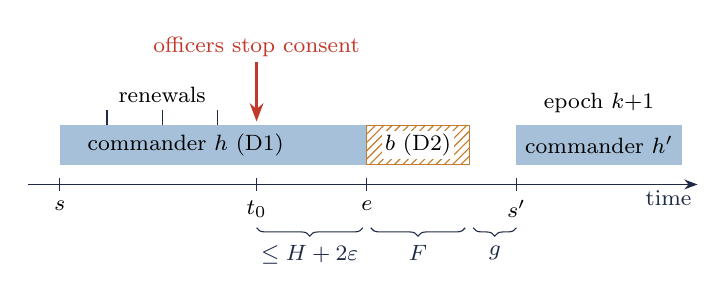
\begin{tikzpicture}[x=1cm,y=1cm,font=\footnotesize,>=Stealth]
  % time axis
  \draw[->,ink] (0,0) -- (8.5,0) node[below left,inner sep=2pt] {time};
  % epoch k: commander
  \fill[accept!55] (0.4,0.25) rectangle (4.3,0.75);
  \node at (2.0,0.5) {commander $h$ (D1)};
  % deputy period
  \fill[pattern=north east lines,pattern color=fence] (4.3,0.25) rectangle (5.6,0.75);
  \draw[fence] (4.3,0.25) rectangle (5.6,0.75);
  \node[fill=white,inner sep=1pt] at (4.95,0.5) {$b$ (D2)};
  % next epoch
  \fill[accept!55] (6.2,0.25) rectangle (8.3,0.75);
  \node at (7.25,0.5) {commander $h'$};
  % renewals
  \foreach \x in {1.0,1.7,2.4} {\draw[ink] (\x,0.75) -- (\x,0.95);}
  \node[above] at (1.7,0.92) {renewals};
  % stop of consent
  \draw[->,warn,thick] (2.9,1.55) -- (2.9,0.8);
  \node[above,warn] at (2.9,1.5) {officers stop consent};
  % ticks
  \foreach \x/\l in {0.4/$s$,2.9/$t_0$,4.3/$e$,6.2/$s'$} {
    \draw[ink] (\x,0.08) -- (\x,-0.08);
    \node[below] at (\x,-0.08) {\l};
  }
  % braces
  \draw[decorate,decoration={brace,mirror,amplitude=3pt},ink] (2.9,-0.55) -- (4.25,-0.55)
    node[midway,below=3pt] {$\le H + 2\eps$};
  \draw[decorate,decoration={brace,mirror,amplitude=3pt},ink] (4.35,-0.55) -- (5.55,-0.55)
    node[midway,below=3pt] {$F$};
  \draw[decorate,decoration={brace,mirror,amplitude=3pt},ink] (5.65,-0.55) -- (6.2,-0.55)
    node[midway,below=3pt] {$g$};
  \node[above] at (7.25,0.78) {epoch $k{+}1$};
\end{tikzpicture}
\caption{Command at one device in epoch $k$ and in the subsequent epoch. From the time
$t_0$, the officers sign no more renewals. The commander $h$ keeps the device until the end
time $e$ of the last renewal. The deputy $b$ can give orders in the period $F$, if
$F > 0$. The new commander $h'$ starts after the guard $g$.}
\label{fig:timeline}
\end{figure}

\section{Analysis of \sys{}}
\label{sec:analysis}

This section shows the properties of \sys{}. All results use the model of \cref{sec:model}:
not more than $f$ officers are hostile, $n \ge 3f + 1$, and
$q = \lceil (n + f + 1)/2 \rceil$. The attacker controls all links in all results. Only for
\cref{thm:tolerance}, it is necessary that messages come through.

\subsection{Two Lemmas}

\begin{lem}[One grant for each epoch]
\label{lem:grant}
A run has not more than one valid grant for each epoch.
\end{lem}

\begin{proof}
Let a run have two different valid grants of an epoch $j > 1$. Each grant has $q$ signers,
thus one loyal officer $u$ signed the two grants. By rule O2, $u$ signs a grant of epoch
$j$ only if $j > E_u$, and then $u$ sets $E_u$ to $j$. The number $E_u$ does not decrease.
Thus $u$ signs not more than one grant of epoch $j$. This is a contradiction.

For epoch 1, the parties have one valid grant at the start. A second valid grant of epoch 1
has a loyal signer, because $q > f$. But a loyal officer signs no grant of epoch 1, because
$E_u \ge 1$ at all times.
\end{proof}

\begin{lem}[Separation]
\label{lem:separation}
Let $\renew{k,e}$ and $\grant{j,h,b,s}$ be valid, with $j > k$. Then $s \ge e + F + g$.
\end{lem}

\begin{proof}
The renewal and the grant have $q$ signers each, thus one loyal officer $u$ signed the two
certificates. First, let $u$ sign the renewal before the grant. Then $M_u \ge e$ when $u$
signs the grant, and rule O2 gives $s \ge M_u + F + g \ge e + F + g$. Second, let $u$ sign
the grant before the renewal, thus $E_u \ge j > k$ from that time. By rule O1, $u$ signs
the renewal only if $k = E_u$. This is a contradiction.
\end{proof}

\subsection{Unity of Command}

\begin{thm}[Unity of command]
\label{thm:unity}
Let $F = 0$ and $g > 2\eps$. Then \sys{} has unity of command with separation
$g - 2\eps$.
\end{thm}

\begin{proof}
Let a device $d$ accept an order of an officer $x$ at real time $t$. Let a device $d'$
accept an order of a different officer $y$ at real time $t'$. Rule D2 does not apply,
because $F = 0$. By rule D1, the orders are for epochs $k$ and $j$, and $x$ and $y$ are the
commanders in valid grants of these epochs. By \cref{lem:grant}, $k \ne j$, because
$x \ne y$. Let $k < j$.

The device $d$ has a valid $\renew{k,e}$ with $C_d(t) \le e$, thus $t \le e + \eps$. The
device $d'$ has a valid $\grant{j,y,b,s}$ with $s \le C_{d'}(t')$, thus $t' \ge s - \eps$.
By \cref{lem:separation}, $s \ge e + g$. Thus $t' - t \ge g - 2\eps$. If $k > j$, the same
argument gives $t - t' \ge g - 2\eps$.
\end{proof}

The theorem applies with a hostile commander, with hostile officers, and with each sequence
of messages. It tells that all orders of one epoch come before all orders of a higher
epoch.

\subsection{Tenure}

\begin{thm}[Tenure of a commander]
\label{thm:tenure}
Let $k$ be an epoch and $t_0$ a real time. Let $W$ be a set of $n - q + 1$ or more loyal
officers. From $t_0$, let no officer in $W$ sign a renewal of epoch $k$. Then no device
accepts an order of the commander for epoch $k$ at a real time $t \ge t_0 + H + 2\eps$.
Also, no device accepts an order of the deputy for epoch $k$ at a real time
$t \ge t_0 + H + F + 2\eps$.
\end{thm}

\begin{proof}
Let $\renew{k,e}$ be a valid renewal. It has $q$ signers, and not more than $q - 1$
officers are not in $W$. Thus one signer $u$ is in $W$. The officer $u$ is loyal, and it
signed at a real time $t_u < t_0$. By rule O1, $e \le C_u(t_u) + H \le t_u + \eps + H$.
Thus $e < t_0 + H + \eps$ for each valid renewal of epoch $k$.

Let a device $d$ accept an order by rule D1 at real time $t$. Then $C_d(t) \le e$ for a
valid renewal, thus $t \le e + \eps < t_0 + H + 2\eps$. Let $d$ accept an order by rule D2
at real time $t$. Then $C_d(t) \le a + F$, and the anchor $a$ is the end time of a valid
renewal. Thus $t < t_0 + H + F + 2\eps$.
\end{proof}

The proof uses no property of the network. The attacker cannot extend the tenure when it
stops, delays or replays messages. It can only make the tenure shorter.

\begin{cor}[Two thresholds]
\label{cor:thresholds}
Let $r_h = n - q + 1$ and $r_l = n - q + 1 - f$.
\begin{enumerate}
  \item If $r_h$ loyal officers stop their consent at $t_0$, the tenure of the commander
  stops before $t_0 + H + 2\eps$. The hostile officers cannot prevent this.
  \item The hostile officers cannot make a valid certificate without $q - f$ loyal signers.
  \item If the number of loyal officers who stop consent is less than $r_l$, then $q$ or
  more loyal officers continue to sign. Thus the renewals continue when the hostile
  officers do not sign.
\end{enumerate}
\end{cor}

\begin{proof}
The first part is \cref{thm:tenure}. The second part is correct because $q > f$. For the
third part, the number of loyal officers is $n - f$ or more. If less than $r_l$ of them
stop, more than $n - f - r_l = q - 1$ continue.
\end{proof}

The two thresholds are different for the two types of commander. To remove a hostile
commander, $r_h$ loyal officers are sufficient. To stop the renewals of a loyal commander,
$r_l$ loyal officers must stop consent, together with $f$ hostile officers. For $n = 3f + 1$
the values are $q = 2f + 1$, $r_h = f + 1$ and $r_l = 1$. Thus one loyal officer and $f$
hostile officers can stop the renewals of a loyal commander. A larger $n$ makes $r_l$
larger: $n = 7$ and $f = 1$ give $q = 5$, $r_h = 3$ and $r_l = 2$.

The numbers of officers for removal and for a new commander are different. For removal,
$r_h$ loyal officers are sufficient. For a new grant, a quorum is necessary. If $r_h$ officers stop
consent and no quorum signs a grant, the system has no commander. Then only local control
stays (rule D3).

\subsection{Outage Tolerance}

\begin{thm}[Outage tolerance]
\label{thm:tolerance}
Let all officers be loyal and give consent to the commander $c$ of an epoch $k$. Let each
officer $u$ have $E_u = k$ and the valid grant of epoch $k$, with the start time $s$. Let
$c$ start a request at intervals of $\Delta$ or less in real time. Let $c$ have the valid
renewal not more than $\delta$ after the start of each request.

Let an outage start at a real time $t_0 \ge s + \Delta + \delta + \eps$. From $t_0$, $c$
and a device $d$ receive only messages that $c$ or $d$ sent, and the switch of $d$ is in
the position ``REMOTE''. Then $d$ accepts each order of $c$ that it receives at a real time
$t$ with $t_0 \le t \le t_0 + H - \Delta - \delta - 4\eps$.
\end{thm}

\begin{proof}
One request started at a real time $t_r$ with $t_0 - \Delta - \delta < t_r \le t_0 -
\delta$. Its end time is $e = C_c(t_r) + H - 2\eps$, thus $e \ge t_r + H - 3\eps$ and
$e \le t_r + H - \eps$. An officer $u$ who receives the request at a real time
$t_u \ge t_r$ has $C_u(t_u) + H \ge t_r - \eps + H \ge e$. Thus each officer can sign by
rule O1, and $c$ has the valid renewal at $t_0$.

Each order of $c$ has the grant and the renewal, and rule D3 does not stop the order. The
device accepts by rule D1 at $t$ if $s \le C_d(t) \le e$. The first condition is
correct because $C_d(t) \ge t_0 - \eps \ge s$. The second condition is correct if
$t + \eps \le e$. This is correct for each $t \le t_r + H - 4\eps$, and
$t_r > t_0 - \Delta - \delta$.
\end{proof}

Thus the outage tolerance of \sys{} is $H - \Delta - \delta - 4\eps$ or more. By
\cref{thm:tenure}, the hostile tenure is not more than $H + 2\eps$. The difference between the
two quantities is not more than $\Delta + \delta + 6\eps$. By \cref{thm:limit}, the
difference cannot be less than zero for a protocol. With the values of \cref{tab:params},
the outage tolerance is 567.2\,s or more. The hostile tenure is not more than 600.4\,s, and the
difference is not more than 33.2\,s.

\subsection{Fallback to the Deputy}

\begin{prp}[Fallback]
\label{prp:fallback}
Let $F > 0$ and $g > 2\eps$. Then \sys{} has these properties.
\begin{enumerate}
  \item At one clock time, one device accepts orders of not more than one officer.
  \item For each epoch, one device accepts orders of the deputy only at clock times in one
  interval of length $F$.
  \item Let a device accept an order of epoch $k$ at real time $t$. Let a device accept an
  order of an epoch $j > k$ at real time $t'$. Then $t' - t \ge g - 2\eps$.
\end{enumerate}
\end{prp}

\begin{proof}
For the first part, let the two orders be for the same epoch. By \cref{lem:grant}, one
order is of the commander and one order is of the deputy. By rule D1, the device has a
valid renewal with an end time $e \ge \tau$. By rule D2, the device has no such renewal.
This is a contradiction.

Then let the orders be for the epochs $k < j$. For the order of epoch $j$, the start time
is $s \le \tau$. For the order of epoch $k$, $\tau \le e + F$ for the end time $e$ of a
valid renewal. By \cref{lem:separation}, $s \ge e + F + g > \tau$. This is a
contradiction.

The second part is correct because the anchor $a$ of an epoch does not change after the
first order of the deputy. Rule D2 accepts an order only if $a < \tau \le a + F$. For the third part, the
order of epoch $k$ gives $t \le e + F + \eps$ for the end time $e$ of a valid renewal. The
order of epoch $j$ gives $t' \ge s - \eps$. By \cref{lem:separation}, $s \ge e + F + g$.
\end{proof}

With $F > 0$, \sys{} does not have unity of command. A device with no new renewal can
accept orders of the deputy while a different device accepts orders of the commander. The
proposition puts a limit on this condition: one interval of length $F$ for each device and
each epoch. The deputy exposure at a device is thus not more than $F + 2\eps$ in real time
for each epoch. By \cref{thm:deputy}, a protocol with the deputy period $F$ cannot have a
smaller exposure.

\section{Cost and Tests}
\label{sec:cost}

This section gives the cost of \sys{} as formulas. It compares \sys{} with four known
designs. It also gives the tests that are done and the tests that are not done.

\subsection{Cost of \sys{}}

\paragraph{Time without command}
Let the commander be loyal, and let an outage of length $\Lambda$ isolate the commander
from each quorum. The commander keeps a device for $H - \Delta - \delta - 4\eps$ or more
(\cref{thm:tolerance}), and for less than $H + 2\eps$. Thus the time without command at the
device is between $\Lambda - H - 2\eps$ and $\Lambda - H + \Delta + \delta + 4\eps$, or zero
if these values are less than zero. If $F > 0$, the deputy can use a period $F$ of this
time.

\paragraph{Time with a hostile commander}
The time is less than $H + 2\eps$ from the time at which $n - q + 1$ loyal officers stop
their consent (\cref{thm:tenure}). The time that is necessary for the officers to make
this decision is not in the formula. The protocol cannot make that time shorter.

\paragraph{Signatures and messages}
For one renewal, one request and $q$ signatures are necessary. Thus the officers make
$q/\Delta$ signatures in a unit of time. A device examines the signatures of a certificate one time,
because it keeps each valid certificate. An order has the grant and one renewal attached,
thus $2q$ signatures. A threshold signature can replace the $q$ signatures of a
certificate. We did not examine that change.

\paragraph{Handover}
A prepared handover has a period of $F + g$ between two commanders (\cref{sec:change}). A
handover that is not prepared has a period of $H + F + g + 2\eps$ or less from the proposal
to the start of the new commander.

\subsection{Four Known Designs}

\Cref{tab:designs} compares \sys{} with four designs. The entries for the four designs come
from their definitions. They do not come from tests.

\begin{description}
  \item[NE] Signed orders with no end time. The device examines only the signature of the
  commander~\cite{saxena2018signature}.
  \item[QO] A quorum for each order. A device accepts an order only with the signatures of
  $q$ officers. A design in which each order goes through replicated servers has the same
  property~\cite{babay2018spire}.
  \item[SL] A lease of length $L$ from one server~\cite{gray1989leases}. The commander
  gets a new lease from the server before the end of each lease.
  \item[TS] Takeover on a timeout $T$. The deputy gets command when no message comes from
  the commander for the time $T$. No quorum signs the takeover, and the command of the
  deputy has no end time.
\end{description}

\begin{table*}[t]
\caption{Four known designs and \sys{}. The quantities are those of
\cref{sec:quantities}. For SL, $L$ is the length of the lease. The last column gives the
weak point of each design.}
\label{tab:designs}
\centering
\small
\begin{tabularx}{\textwidth}{@{}ll>{\raggedright\arraybackslash}X>{\raggedright\arraybackslash}p{0.13\textwidth}l>{\raggedright\arraybackslash}X@{}}
\toprule
Design & Outage tolerance & Hostile tenure & Deputy exposure & Signatures & Weak point \\
\midrule
NE & No limit & No limit & None & 1 for each order & A hostile commander stays (\cref{thm:limit}) \\
QO & Zero & Zero & None & $q$ for each order & No command in an outage \\
SL & $L - \Delta - \delta - 4\eps$ & $L + 2\eps$, or no limit with the key of the server & None & 1 for each renewal & One server \\
TS & No limit & No limit & No limit & 1 for each order & The timeout attack (\cref{thm:deputy}) \\
\sys{} & $H - \Delta - \delta - 4\eps$ & $H + 2\eps$ & $F + 2\eps$ for each epoch & $q$ for each renewal & No command after $H$ in an outage \\
\bottomrule
\end{tabularx}
\end{table*}

Three points follow from the table. First, expiry has the same cost in SL and in \sys{}.
For $L = H$, the two designs have the same time without command when the commander cannot
get a renewal.

Second, \sys{} is better than SL in two properties. No one key gives the attacker a tenure
with no limit. Also, the officers of a quorum can be at different locations. Some of them
can be on the same side of a cut as the commander. Third, only \sys{} puts a limit on the
timeout attack.

\Cref{fig:tradeoff} shows the two quantities of \cref{thm:limit}. No protocol is below the
diagonal. \sys{} is above the diagonal by $\Delta + \delta + 6\eps$ or less. The designer
moves along this line when the designer selects $H$.

\begin{figure}[t]
\centering
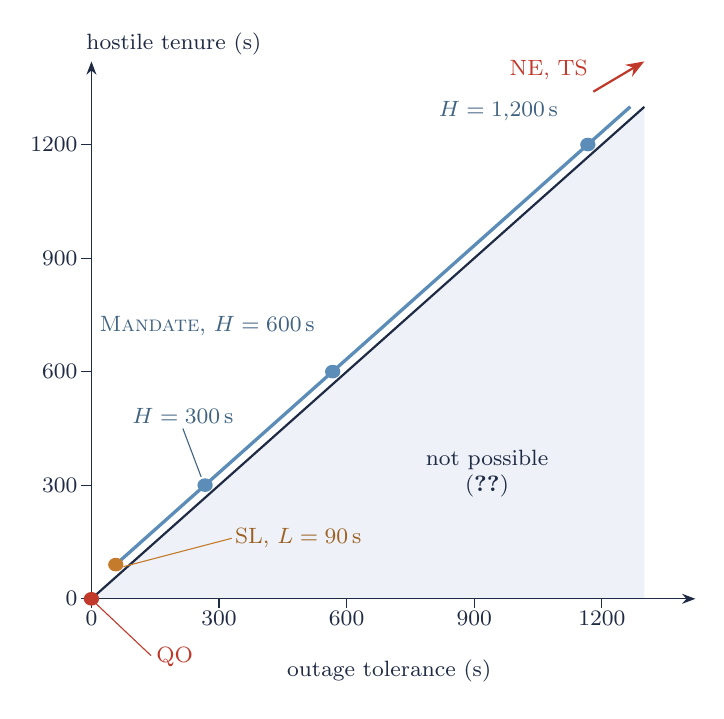
\begin{tikzpicture}[x=0.0054cm,y=0.0048cm,font=\footnotesize,>=Stealth]
  % axes: 0..1400 s
  \fill[soft] (0,0) -- (1300,0) -- (1300,1300) -- cycle;
  \draw[->,ink] (0,0) -- (1420,0);
  \node[ink] at (700,-190) {outage tolerance (s)};
  \draw[->,ink] (0,0) -- (0,1420) node[above right,inner sep=2pt,xshift=-4pt] {hostile tenure (s)};
  \foreach \v in {0,300,600,900,1200} {
    \draw[ink] (\v,0) -- (\v,-25) node[below,inner sep=1pt] {\v};
    \draw[ink] (0,\v) -- (-25,\v) node[left,inner sep=1pt] {\v};
  }
  % diagonal: the limit
  \draw[ink,thick] (0,0) -- (1300,1300);
  \node[align=center,ink] at (930,330) {not possible\\(\cref{thm:limit})};
  % Mandate line: tenure = tolerance + 33.2 s
  \draw[accept,very thick] (57,90.4) -- (1267,1300.4);
  \foreach \h in {300,600,1200} {
    \fill[accept] (\h-32.8,\h+0.4) circle[radius=18];
  }
  \node[accept!70!black,anchor=east] at (548,720) {\sys{}, $H = 600$\,s};
  \draw[accept!70!black] (258,322) -- (215,450);
  \node[accept!70!black,anchor=south,inner sep=1pt] at (215,455) {$H = 300$\,s};
  \node[accept!70!black,anchor=east] at (1120,1290) {$H = 1{,}200$\,s};
  % QO at the origin
  \fill[warn] (0,0) circle[radius=18];
  \draw[warn] (10,-12) -- (140,-150);
  \node[warn,anchor=west,inner sep=1pt] at (145,-155) {QO};
  % SL with L = 90 s
  \fill[fence] (57.2,90.4) circle[radius=18];
  \draw[fence] (75,85) -- (330,160);
  \node[fence!80!black,anchor=west,inner sep=1pt] at (330,160) {SL, $L = 90$\,s};
  % NE and TS: no limit
  \draw[->,warn,thick] (1180,1340) -- (1300,1420);
  \node[warn,anchor=south east] at (1190,1345) {NE, TS};
\end{tikzpicture}
\caption{Hostile tenure and outage tolerance. The gray area is not possible for a protocol
(\cref{thm:limit}). The points for \sys{} use the values of \cref{tab:params}. The point
for SL applies only if the server is loyal. NE and TS have no limit.}
\label{fig:tradeoff}
\end{figure}

\subsection{Cost of Expiry and of Timeouts with No Attacker}
\label{sec:baseline}

The previous draft of this work has a simulation model of incident
response~(\file{testbed/} in the repository). The model has a commander, a deputy,
vehicles at an incident, and a server at a regional center. It has no hostile officer, and
it is not a model of a power grid. Its \tbTotalRuns{} runs give two results that apply
here. \pending{The numbers of this subsection come from the previous model. A simulation
with a hostile commander is not done at this time.}

The first result is the cost of expiry. In one condition, all vehicles are isolated from
the server for 1{,}200\,s, and the commander is loyal and has links to the vehicles. With a
lease of 90\,s from the server (design SL), the system was without command for
\tbPBNoCommand{} of the outage. The device of the commander rejected \tbPBRefused{} correct
orders. These values are medians of \tbSeedsPerCell{} runs. The formula of this section
gives $1{,}200 - 90 = 1{,}110$\,s or more for the same condition.

For \sys{} in that condition, the formulas give these values. With $H = 600$\,s, the time
without command is between 600\,s and 633\,s. With $H = 1{,}233$\,s or more, it is zero,
and the hostile tenure is then 1{,}200\,s or more (\cref{thm:limit}). If a quorum of
officers is on the same side of the cut as the commander, the time without command is zero
for each $H$. We calculated these values. They are not results of a simulation.

The second result is about timeouts. With a takeover on a timeout (design TS), one delayed
message caused two commanders at the same time for a median of \tbRelayOverlap{}. No
attacker was in that run. With the acknowledged timeout of the previous draft, the value
was \tbRelayOverlapAcked{}. Thus a timeout can give command to two persons when no party is
hostile.

\subsection{Random Tests of the Rules}
\label{sec:random}

We wrote a program that makes random runs of the rules O1, O2, D1 and
D2~(\file{paper/model/mandate_sim.py}). In each run, a hostile officer signs each
certificate with a probability of 0.8, and loyal officers stop their consent at random
times. The attacker gives valid certificates to three devices at random times. After each
step, the program examines \cref{lem:grant}, \cref{lem:separation}, \cref{thm:unity},
\cref{thm:tenure} and the first two parts of \cref{prp:fallback}.

With the rules of the paper, the program found no failure in 3{,}000 runs of 400 steps
each. The runs use $(n, f)$ from $(4,1)$, $(5,1)$, $(7,2)$ and $(10,3)$. The other values
are $H = 60$, $g = 1$, $\eps = 0.4$, and $F = 0$ or $F = 20$.

The program found failures when we removed one condition from the rules. Without the start
time in rule O2, 974 of the 3{,}000 runs had a failure. Without the epoch in rule O2, all
3{,}000 runs had a failure. Without the epoch and the end time in rule O1, 2{,}992 runs
had a failure. With a quorum of a majority only, 903 runs had a failure.

These tests are not a proof and not a model check. The rules, the proofs
and the program also have one source. Thus the tests cannot find an error that is in all
three.

\subsection{Tests That Are Not Done}
\label{sec:plan}

Four tests are necessary before a submission. \pending{None of the four is done at this
time.}

\begin{description}
  \item[E1] \emph{Model check.} Write the rules in TLA+~\cite{tlaplus} and examine them with the
  TLC model checker. The model has four officers, one hostile officer, two devices and a
  clock with steps. The attacker can give each valid certificate to each device at each
  step. The properties are those of \cref{lem:grant}, \cref{lem:separation},
  \cref{thm:unity}, \cref{thm:tenure} and \cref{prp:fallback}.
  \item[E2] \emph{Simulation with an attacker.} Add a hostile commander, a hostile deputy and an
  attacker on the links to the simulation model, for the five designs of
  \cref{tab:designs}. Use four conditions: an outage with a loyal commander, a hostile
  commander with a cut, the timeout attack, and a commander who stops. Use $H$ of 90, 300, 600 and
  1{,}200\,s, and $F$ of 0, 60 and 120\,s. Use outages of 300, 1{,}200 and 3{,}600\,s, and
  20 runs for each condition. Measure the hostile tenure, the time without command, the
  deputy exposure, and the number of loyal commanders that the officers remove.
  \item[E3] \emph{Check by a power engineer.} Examine four items with a power engineer in
  one hour. The items are the grid example, rule D3, the usual length of an outage, and the
  source of time in a substation.
  \item[E4] \emph{Full text.} Read the full text of each source in \cref{tab:position} and
  correct the table.
\end{description}

Test E2 has four hypotheses. First, for each design, the hostile tenure is not less than
the outage tolerance (\cref{thm:limit}). Second, for \sys{}, the hostile tenure is less than
$H + 2\eps$ in each run (\cref{thm:tenure}). Third, for \sys{} with $F = 0$, no run has
two commanders at the same time, and for TS the timeout attack gives command to the deputy
(\cref{thm:unity,thm:deputy}). Fourth, the time without command for \sys{} agrees with the
formula of this section. A result against one of the first three hypotheses shows an error
in a proof or in the program.

\section{Discussion}
\label{sec:discussion}

\subsection{How to Select a Design}
\label{sec:select}

The limits of \cref{sec:limits} tell when each design of \cref{tab:designs} is the correct
selection.

\begin{itemize}
  \item Use QO if each order can wait until a quorum signs it. Then the hostile tenure is
  zero, and no other design is safer.
  \item Use SL if no officer can be hostile, and the attacker cannot get the key of the
  server. Then one server is sufficient.
  \item Use NE if each order is easy to cancel and the system has a record of all orders.
  Then a long hostile tenure causes small damage.
  \item Use \sys{} if the commander must continue through outages, an officer can be
  hostile, and orders can cause damage that is not easy to repair.
\end{itemize}

A designer who selects \sys{} makes three decisions. The first decision is the horizon
$H$. It is the longest outage that a loyal commander must continue through. It is also the
time that a hostile commander keeps a device, and no protocol can change this
(\cref{thm:limit}). Thus the designer compares two risks: a time $H$ with a hostile
commander, and an outage longer than $H$ with only local control.

The second decision is the fallback period $F$. With $F = 0$, the system has unity of
command, and it has no commander between the end of the last renewal and a new grant. With
$F > 0$, the deputy can give orders in that period, and a hostile deputy gets the same
period at each device.

The third decision is the quorum $q$. The value $q = \lceil (n + f + 1)/2 \rceil$ is the
minimum. A larger $q$, to a maximum of $n - f$, makes the two thresholds of
\cref{cor:thresholds} smaller. Then a smaller group of loyal officers can remove a hostile
commander. But a smaller group of loyal officers, together with the hostile officers, can
also stop the renewals of a loyal commander.

\subsection{Limits of the Model}
\label{sec:model-limits}

\paragraph{Clocks}
The tenure limit uses the clock of the device. An attacker who sets that clock to a previous time extends the tenure. Substations frequently get time from satellite signals, and an
attacker can forge such signals~\cite{zhang2013tsa,gao2023quick}. Methods to find such an
attack are known~\cite{laverty2022gnss}. A device must thus keep a local clock, and
$\eps$ must include the error of that clock during the longest outage. \pending{Not done at
this time: a model of clock attacks.}

\paragraph{More than $f$ hostile officers}
If more than $f$ officers are hostile, it is possible that each officer who is in two
quorums is hostile. Then \cref{lem:grant} and \cref{lem:separation} are not correct, and two commanders
are possible. With $q$ hostile officers, no property stays.

\paragraph{A constant set of officers}
The set of officers and their keys do not change in the model. A change of that set is a
different problem~\cite{kuznetsov2022reconfig}. We did not examine it.

\paragraph{Hostile devices}
Each device is correct in the model. A device with changed software can do each order and
can ignore each rule. The report on the 2015 attack records an attack on the firmware of
network devices at substations~\cite[p.~9]{eisac2016ukraine}.

\paragraph{The decision to stop consent}
The model does not tell how an officer knows that a commander is hostile. A second
channel, for example a telephone, helps the officers to make that decision. An attacker can
also attack that channel. The telephone calls of the 2015 attack are an
example~\cite[p.~2]{eisac2016ukraine}.

\paragraph{Damage in the tenure}
\sys{} puts a limit on the time of a hostile commander, and not on the damage. In that
time, the hostile commander can give each order. Checks of the contents of
orders~\cite{mashima2018onthefly,hong2019resilient} and a limit on the number of orders
decrease the damage. \Cref{thm:limit} shows that such checks cannot make the tenure
shorter.

\paragraph{A faster stop when messages come through}
A device that receives a valid grant of a higher epoch can reject the orders of the
previous epoch immediately. This rule is safe, because a quorum signs each valid grant. It
makes the tenure shorter when the attacker does not stop the grant. \Cref{thm:limit} shows
that a design cannot use this rule as a replacement for expiry.

\paragraph{An attacker who only stops messages}
An attacker who controls the links can always stop orders and renewals. Expiry thus gives
that attacker no new method to stop command. A takeover on a timeout is different: it
gives the attacker a method to move command.

\subsection{Known Risks of Errors in This Draft}

Five risks are known. First, no second person and no model checker examined the proofs.
Second, the data about related work come from abstracts, and \cref{tab:position} can
be incorrect for a source. Third, the entries of \cref{tab:designs} for the four known
designs come from definitions and not from tests. Fourth, no power engineer examined the
grid example and rule D3. Fifth, the numbers of \cref{sec:baseline} come from a model of
incident response with no attacker.

\section{Conclusion}
\label{sec:conclusion}

A device that obeys an isolated commander cannot know if that commander is loyal. This
paper gives the cost of that fact. For each protocol, a hostile commander keeps a device
for a time that is not less than the outage tolerance. A deputy period is in the same
condition: an attacker with the key of the deputy gets the same period.

\sys{} is a protocol that is near these limits. A quorum of officers signs each renewal of
command, and each device compares the end time with its clock. Thus the officers remove a
commander without a message to the device. The hostile officers cannot prevent this, and
they cannot make a valid certificate without loyal signers. The hostile tenure is more than the outage tolerance by the renewal interval,
the collection time and six clock errors, or less.

The proofs are in this paper. Four checks are not done at this time. They are a model
check, a simulation with a hostile commander, a check by a power engineer, and a full-text
check of the related work.


\ifsrds
  \appendices
  \section{Record of the Search}
\label{app:search}

We did the search on 10 November 2026 with the Consensus search engine. Each query gave 20
records, and we used no filter. We examined the title and the abstract of each of the 300
records, and we kept approximately 75 records. The paper refers to the records that are
related to one of the six properties of \cref{tab:position}. \Cref{tab:queries} gives the
text of each query.

\begin{table*}[t]
\caption{The 15 queries of the search. Each query gave 20 records. The right column gives
the result of the query for this paper.}
\label{tab:queries}
\centering
\footnotesize
\begin{tabularx}{\textwidth}{@{}l>{\raggedright\arraybackslash}p{0.52\textwidth}>{\raggedright\arraybackslash}X@{}}
\toprule
No. & Text of the query & Result \\
\midrule
1 & ``threshold multi-party authorization of critical control commands in SCADA or smart grid to tolerate a compromised operator or insider'' & Checks of one order, and two designs with a quorum or a second factor \\
2 & ``localized threshold certificate renewal with ticket expiry for access control in mobile ad hoc networks'' & Threshold certificates with expiry, and no commander \\
3 & ``tolerating Byzantine faulty clients in quorum systems: limiting writes after a faulty client is removed'' & A limit on the writes of a removed client \\
4 & ``intrusion-tolerant SCADA for power grid substations: Byzantine resilience, compromised operator or HMI outside the threat model'' & Hostile servers, and a loyal operator \\
5 & ``trade-off between availability during network partition and timely revocation of authorization: bounded staleness, stale-safe access decisions'' & The problem, and no quantity for command \\
6 & ``leases under Byzantine faults: bounding how long a compromised leader or primary keeps authority'' & A leader with no authority without a quorum \\
7 & ``transfer of control authority between human operators in control rooms or SCADA: shift handover, operator authority transfer under degraded communication'' & Loyal parties in all 20 records \\
8 & ``revocation for offline or partitioned devices: short-lived credentials versus revocation lists in IoT and cyber-physical systems'' & A maximum for the time after revocation (HRCred) \\
9 & ``command authentication at the substation when the control center is compromised: verify legitimacy of remote control commands before execution'' & Checks of the sender and of the contents of one order \\
10 & ``two-person rule or dual authorization for critical control commands in industrial control systems and SCADA'' & Models of access control and surveys, and no rule for two persons \\
11 & ``attacker-induced failover or leader change: network adversary delays heartbeats to trigger takeover; partition attacks on failure detection and leader election'' & Incorrect timeouts as an attack on the speed of replication \\
12 & ``time synchronization attack or GPS spoofing against clocks in power grid substations and control systems: effect on time-based security mechanisms'' & Attacks on the time source of a substation \\
13 & ``delegation of launch authority and the always/never dilemma in nuclear command and control: positive and negative control'' & The same problem, and no protocol model \\
14 & ``manual operation and local control of substations as fallback after loss of SCADA in a cyber attack: restoration, Ukraine 2015 lessons'' & Attacks on substations, and surveys \\
15 & ``Byzantine fault tolerant access control and revocation in decentralized collaboration with compromised administrators'' & Access control without a quorum \\
\bottomrule
\end{tabularx}
\end{table*}

The search has three limits. First, one search engine gave all records. Second, we read
abstracts and not the full text. Third, no second person examined the selection of the
records.

  \section*{Acknowledgment}
  The work presented in this paper was supported by Digitala Stambanan IndTech (Vinnova
  Reference Number: 2024-02510), and the Horizon Europe projects COP-PILOT under grant
  agreement 101189819 and RemaNet under grant agreement 101138627.
  \bibliographystyle{IEEEtran}
  \bibliography{refs}
\else
% acmart reads the acks environment line by line in review mode: \begin{acks} and \end{acks}
% must start at the left margin, each on its own line.
\begin{acks}
  The work presented in this paper was supported by Digitala Stambanan IndTech (Vinnova
  Reference Number: 2024-02510), and the Horizon Europe projects COP-PILOT under grant
  agreement 101189819 and RemaNet under grant agreement 101138627.
\end{acks}
  \bibliographystyle{ACM-Reference-Format}
  \bibliography{refs}
  \appendix
  \section{Record of the Search}
\label{app:search}

We did the search on 10 November 2026 with the Consensus search engine. Each query gave 20
records, and we used no filter. We examined the title and the abstract of each of the 300
records, and we kept approximately 75 records. The paper refers to the records that are
related to one of the six properties of \cref{tab:position}. \Cref{tab:queries} gives the
text of each query.

\begin{table*}[t]
\caption{The 15 queries of the search. Each query gave 20 records. The right column gives
the result of the query for this paper.}
\label{tab:queries}
\centering
\footnotesize
\begin{tabularx}{\textwidth}{@{}l>{\raggedright\arraybackslash}p{0.52\textwidth}>{\raggedright\arraybackslash}X@{}}
\toprule
No. & Text of the query & Result \\
\midrule
1 & ``threshold multi-party authorization of critical control commands in SCADA or smart grid to tolerate a compromised operator or insider'' & Checks of one order, and two designs with a quorum or a second factor \\
2 & ``localized threshold certificate renewal with ticket expiry for access control in mobile ad hoc networks'' & Threshold certificates with expiry, and no commander \\
3 & ``tolerating Byzantine faulty clients in quorum systems: limiting writes after a faulty client is removed'' & A limit on the writes of a removed client \\
4 & ``intrusion-tolerant SCADA for power grid substations: Byzantine resilience, compromised operator or HMI outside the threat model'' & Hostile servers, and a loyal operator \\
5 & ``trade-off between availability during network partition and timely revocation of authorization: bounded staleness, stale-safe access decisions'' & The problem, and no quantity for command \\
6 & ``leases under Byzantine faults: bounding how long a compromised leader or primary keeps authority'' & A leader with no authority without a quorum \\
7 & ``transfer of control authority between human operators in control rooms or SCADA: shift handover, operator authority transfer under degraded communication'' & Loyal parties in all 20 records \\
8 & ``revocation for offline or partitioned devices: short-lived credentials versus revocation lists in IoT and cyber-physical systems'' & A maximum for the time after revocation (HRCred) \\
9 & ``command authentication at the substation when the control center is compromised: verify legitimacy of remote control commands before execution'' & Checks of the sender and of the contents of one order \\
10 & ``two-person rule or dual authorization for critical control commands in industrial control systems and SCADA'' & Models of access control and surveys, and no rule for two persons \\
11 & ``attacker-induced failover or leader change: network adversary delays heartbeats to trigger takeover; partition attacks on failure detection and leader election'' & Incorrect timeouts as an attack on the speed of replication \\
12 & ``time synchronization attack or GPS spoofing against clocks in power grid substations and control systems: effect on time-based security mechanisms'' & Attacks on the time source of a substation \\
13 & ``delegation of launch authority and the always/never dilemma in nuclear command and control: positive and negative control'' & The same problem, and no protocol model \\
14 & ``manual operation and local control of substations as fallback after loss of SCADA in a cyber attack: restoration, Ukraine 2015 lessons'' & Attacks on substations, and surveys \\
15 & ``Byzantine fault tolerant access control and revocation in decentralized collaboration with compromised administrators'' & Access control without a quorum \\
\bottomrule
\end{tabularx}
\end{table*}

The search has three limits. First, one search engine gave all records. Second, we read
abstracts and not the full text. Third, no second person examined the selection of the
records.

\fi

\end{document}
